% Phase 1 handout -- RISC-V RV32I Assembly and Assembler
% EEL 4768 Computer Architecture, Fall 2026
%
% NOTE TO INSTRUCTOR (delete before distributing, or keep as a LaTeX comment):
% This revision restructures the original phase_1.pdf and adds worked
% examples, an address-map figure, a register table, and several
% "Clarification" boxes. Every clarification box is grounded in the actual
% skeleton files and the self-check harness under phase_1/source_test/
% (grade_test.py, config.py, splice.py, tests/all_instructions.s), NOT in
% assumptions. Three are worth your explicit sign-off before this goes out:
%   1. Output file names (Section 5.2): config.py's ASSEMBLER_OUTPUTS maps
%      the instruction files to "<name>.hex.txt" / "<name>.bin.txt", NOT
%      "<name>_instr.hex.txt" as the original table's filenames read. I
%      corrected the table to match the checker. Please confirm the live
%      Gradescope autograder agrees before students see this.
%   2. Sobel G_y sign (Section 4.3): source_test/configs/sobel/1.data and
%      skeletons/sobel.s both define g_y as [[1,2,1],[0,0,0],[-1,-2,-1]],
%      the negation of the G_y formula in the original handout. I flagged
%      this rather than silently "fixing" the formula, since I can't tell
%      which one is the intended convention -- please pick one and make the
%      formula and the data agree.
%   3. The worked convolution example in the original PDF (page 5) sums the
%      nine products to "4"; the arithmetic as printed (with two sign typos
%      and an extra term) actually sums to 8. I recomputed it directly in
%      Section 4.3's worked example and it comes out to 8 -- double-check
%      my arithmetic, but I believe the original's "4" was itself a typo.

\documentclass[11pt]{article}

\usepackage[letterpaper,margin=1in]{geometry}
\usepackage{amsmath,amssymb}
\usepackage{booktabs}
\usepackage{array}
\usepackage{multirow}
\usepackage{caption}
\usepackage{xcolor}
\usepackage{enumitem}
\usepackage{tikz}
\usetikzlibrary{arrows.meta,positioning,calc}
\usepackage{listings}
\usepackage[most]{tcolorbox}
\usepackage{fancyhdr}
\usepackage{parskip}
\usepackage[colorlinks=true,linkcolor=blue!50!black,urlcolor=blue!50!black]{hyperref}

\setlist[itemize]{topsep=2pt,itemsep=2pt,parsep=0pt}
\setlist[enumerate]{topsep=2pt,itemsep=2pt,parsep=0pt}

\lstset{
  basicstyle=\ttfamily\small,
  frame=single,
  breaklines=true,
  columns=fullflexible,
  keepspaces=true,
  showstringspaces=false,
  tabsize=4,
  backgroundcolor=\color{black!3}
}

\tcbuselibrary{skins,breakable}

\newtcolorbox{important}{
  colback=red!5!white, colframe=red!55!black, breakable,
  fonttitle=\bfseries, title=Note
}
\newtcolorbox{clarification}{
  colback=blue!5!white, colframe=blue!45!black, breakable,
  fonttitle=\bfseries, title=Clarification
}
\newtcolorbox{pitfall}{
  colback=orange!8!white, colframe=orange!65!black, breakable,
  fonttitle=\bfseries, title=Common Pitfall
}
\newtcolorbox{worked}{
  colback=green!5!white, colframe=green!35!black, breakable,
  fonttitle=\bfseries, title=C Example
}
\newtcolorbox{example}{
  colback=green!5!white, colframe=green!35!black, breakable,
  fonttitle=\bfseries, title=Breakdown
}

\setlength{\headheight}{14pt}
\emergencystretch=1.5em

\pagestyle{fancy}
\fancyhf{}
\fancyhead[L]{EEL 4768 -- Computer Architecture}
\fancyhead[R]{Phase 1: RISC-V RV32I Assembly and Assembler}
\fancyfoot[C]{\thepage}
\renewcommand{\headrulewidth}{0.4pt}

\title{\vspace{-1.5cm}\textbf{Phase 1}\\[2pt]\Large RISC-V RV32I Assembly and Assembler}
\author{EEL 4768 Computer Architecture \\ Fall 2026}
\date{}

\begin{document}
\maketitle
\thispagestyle{fancy}
\vspace{-1cm}

\section*{Learning Objectives}
By the end of this phase you should be able to:
\begin{itemize}
  \item Read and write RV32I assembly by hand, using only the base integer
        instruction set.
  \item Explain how a RISC-V instruction is encoded as a 32-bit word, and
        how that word is serialized to bytes in memory.
  \item Build a two-pass assembler (labels/symbol table, then encode) that
        handles the \emph{entire} RV32I base ISA, not just the sample
        programs you were given.
\end{itemize}

\begin{important}
You may \textbf{only use instructions from the base RV32I ISA} in this phase -- for both Part 1 and Part 2. See The RV32I reference card on
Webcourses for the list of allowed instructions. Additionally, every program must
terminate with \texttt{ecall} (see \texttt{examples/addition.s}), and your assembler should be able to compile this instruction.
\textbf{Using any instruction outside base RV32I earns a zero on that
problem}, even if the program otherwise produces the right answer.
\end{important}

\section{Submission}
\begin{itemize}
\item \textbf{One submission per group.} In this phase, you will manually submit your work to webcourses as a zip file. Students in multiple groups, or not in a group by the time of submission, will receive \textbf{no credit} for the submission.
%   \item \textbf{One submission per group.} Use Gradescope's
%         \emph{``View or Edit Group''} to add every teammate to the same
%         submission, and double-check that this matches your assigned group
%         on Webcourses. A student who is missing from the Gradescope group,
%         or added to a group they don't belong to, gets \textbf{no credit}
%         for the submission -- Gradescope does not reconcile this for you.
  \item \textbf{Files to submit}:
\begin{lstlisting}
gemm.s
mult.s
sobel.s
assembler.py
any additional files needed for your assembler
\end{lstlisting}
        Start each \texttt{.s} file from its skeleton in
        \texttt{phase\_1/skeletons/} and \texttt{assembler.py} from
        \texttt{phase\_1/skeletons/assembler.py}.
\end{itemize}

\section{Grading Rubric}
\label{sec:rubric}
\begin{center}
\begin{tabular}{@{}llr@{}}
\toprule
\textbf{Category} & \textbf{Problem} & \textbf{Points} \\
\midrule
\multirow[t]{4}{*}{RISC-V Assembly}
  & Multiplication      & 0.5 \\
  & GEMM                & 0.5 \\
  & Sobel               & 0.5 \\
  & \textit{subtotal}   & \textit{1.5} \\
\midrule
\multirow[t]{5}{*}{Assembler}
  & Multiplication      & 0.166 \\
  & GEMM                & 0.166 \\
  & Sobel               & 0.166 \\
  & Instruction Test    & 1.0 \\
  & \textit{subtotal}   & \textit{1.5} \\
\midrule
\textbf{Total} & & \textbf{3.0} \\
\bottomrule
\end{tabular}
\end{center}

% \begin{clarification}
% \textbf{What is the ``Instruction Test''?} It is the single largest item
% on this phase -- 1.0 of the 1.5 assembler points, two-thirds of your
% assembler grade and about \emph{double} the other three assembler problems
% combined -- so budget your time accordingly. It assembles one program that
% exercises \emph{every} RV32I instruction and format (R/I/S/B/U/J), using
% both numeric register names (\texttt{x0}--\texttt{x31}) and ABI names
% (\texttt{a0}, \texttt{sp}, \texttt{ra}, \ldots), forward and backward
% labels, and positive and negative immediates at their encodable extremes.

% \textbf{You already have this program.} The copy the local self-check runs
% ships in the repository at
% \texttt{phase\_1/\allowbreak source\_test/\allowbreak tests/\allowbreak all\_instructions.s}.
% Read it early: it is the clearest available specification of what your
% assembler must handle, and every requirement listed in
% Section~\ref{sec:assembler-reqs} is visible in it. Passing it means your
% assembler is a real, general RV32I assembler -- not a special case for
% \texttt{addition.s} plus the three problems below. See
% Section~\ref{sec:regnames} for the register-name table.
% \end{clarification}

\section{Memory Layout}
\label{sec:memlayout}
This phase, and future phases, uses a memory layout where instructions start at
\texttt{0x00400000} and the program's data starts at
\texttt{0x10010000}.

\begin{center}
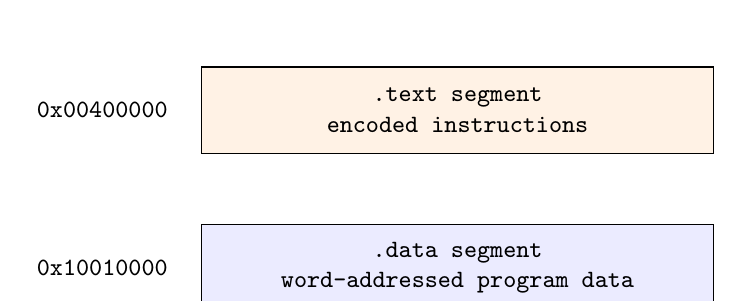
\begin{tikzpicture}[
  seg/.style={draw, minimum width=6.5cm, minimum height=1.1cm, align=center, font=\ttfamily\small},
  lbl/.style={font=\small}
]
\node[seg, fill=orange!10] (instr) at (0,0) {\texttt{.text} segment\\encoded instructions};
\node[lbl, left=0.3cm of instr] {\texttt{0x00400000}};
\node[seg, fill=blue!8] (data) at (0,-2) {\texttt{.data} segment\\word-addressed program data};
\node[lbl, left=0.3cm of data] {\texttt{0x10010000}};
\end{tikzpicture}
\end{center}

\begin{important}
Your assembler must place \texttt{.data} at \texttt{0x10010000} and
\texttt{.text} at \texttt{0x00400000} \emph{exactly}. Any address
arithmetic your encoded program relies on, such as branching, jumping, loading, and storing will compute with this assumption.
\end{important}

\newpage

\section{Part 1: RISC-V Assembly}
\label{sec:part1}

Each problem provides a skeleton RISC-V assembly file (.s) with a pre-populated .data section containing an example input, a zeroed output, and a main: label. Write your program starting at main: and terminate using ecall, as demonstrated in addition.s.

\begin{important}
The numbers in your skeleton's \texttt{.data} section (e.g.\ \texttt{a: .word 22}
in \texttt{mult.s}) are just \emph{one} example configuration. Final grading will use multiple configurations design to stress test your program.
\end{important}

\subsection{Multiplication}
Multiply two words \texttt{a} and \texttt{b}, storing the result in
\texttt{c}. The base RV32I ISA has no multiply instruction, so you must build one out
of shifts and adds. You will be tasked with implementing a \textbf{bit-serial
multiplication algorithm}. Each loop examines one bit of $B$ at a time. When $B_i = 1$, a shifted value of A is accumulated ($A \ll i$). This can be formulated as:
\[C = A \times B, \qquad C = \sum_{i=0}^{N-1} B_i \,(A \ll i) \]

\begin{worked}
\begin{lstlisting}[language=C]
for(i = 0; i < 32; i++):
      C += B * (A << i)
\end{lstlisting}
\end{worked}

\newpage

\subsection{General Matrix Multiplication (GEMM)}
Compute the GEMM of two $4\times4$ matrices \texttt{a} and \texttt{b},
storing the $4\times4$ result in \texttt{c}:
\[
\begin{bmatrix} C_{11} & \cdots & C_{1j} \\ \vdots & \ddots & \vdots \\ C_{i1} & \cdots & C_{ij} \end{bmatrix}
=
\begin{bmatrix} A_{11} & \cdots & A_{1k} \\ \vdots & \ddots & \vdots \\ A_{i1} & \cdots & A_{ik} \end{bmatrix}
\times
\begin{bmatrix} B_{11} & \cdots & B_{1j} \\ \vdots & \ddots & \vdots \\ B_{k1} & \cdots & B_{kj} \end{bmatrix},
\qquad
C_{ij} = \sum_{k=0}^{K-1} A_{ik} \times B_{kj}
\]
with $M{=}N{=}K{=}4$. Use exactly this loop ordering ($m$, then $n$, then
$k$):

\begin{worked}
\begin{lstlisting}[language=C]
for (m = 0; m < M; m++) {
  for (n = 0; n < N; n++) {
    for (k = 0; k < K; k++) {
      C[m,n] += A[m,k] * B[k,n];
    }
  }
}
\end{lstlisting}
\end{worked}

The skeleton stores each matrix as \textbf{16 consecutive words in
row-major order} (row 0's four words, then row 1's, \ldots), not as a true
2D structure -- there is no RV32I ``2D array.'' You must convert a $(row,
col)$ index into a byte offset yourself.

\newpage

\subsection{Sobel Filter}
The Sobel filter approximates the horizontal and vertical intensity
gradient of an image by convolving it with two $3\times3$ kernels,
$G_x$ and $G_y$:
\[
G_x = \begin{bmatrix} -1 & 0 & +1 \\ -2 & 0 & +2 \\ -1 & 0 & +1 \end{bmatrix}
\qquad
G_y = \begin{bmatrix} -1 & -2 & -1 \\ 0 & 0 & 0 \\ +1 & +2 & +1 \end{bmatrix}
\]

\begin{important}
\textbf{Use the kernel values exactly as given in your skeleton's
\texttt{.data} section, not from memory of the formula above.} The
provided \texttt{sobel.s} skeleton (and the grading data) define
\texttt{gy} as \texttt{[[1,2,1],\allowbreak[0,0,0],\allowbreak[-1,-2,-1]]}, which differs from the kernels above to more thoroughly test your convolution logic.
\end{important}

Convolving a $3\times3$ kernel over a $5\times5$ image with stride 1
produces a $3\times3$ output: at each of the 9 output positions, take the
element-wise product of the kernel with the $3\times3$ window of the image
under it, and sum the 9 products.

\begin{example}
Given the $5\times5$ image $A$ and kernel $B$ below, and the top-left
$3\times3$ window $A_{w0}$:
\[
A = \begin{bmatrix} 4&5&1&2&3 \\ 3&0&1&3&5 \\ 4&6&7&3&1 \\ 2&1&0&8&9 \\ 3&6&6&3&4 \end{bmatrix}
\qquad
B = \begin{bmatrix} -1&-2&-1 \\ 0&0&0 \\ +1&+2&+1 \end{bmatrix}
\qquad
A_{w0} = \begin{bmatrix} 4&5&1 \\ 3&0&1 \\ 4&6&7 \end{bmatrix}
\]
Element-wise product of $A_{w0}$ and $B$, summed:
\begin{align*}
&(4)({-}1) + (5)({-}2) + (1)({-}1) + (3)(0) + (0)(0) + (1)(0) + (4)(1) + (6)(2) + (7)(1) \\
&\quad = -4-10-1+0+0+0+4+12+7 = 8
\end{align*}
so the first output element is $8$. Slide the window one column right
(stride 1) to get the next output element, wrapping to the next row after
the last column, until all 9 output positions are filled. Do this
independently for $G_x$ and $G_y$, then add the two $3\times3$ results
element-wise to get the final output:
\[
C_{i,j} = \mathtt{gx}_{i,j} + \mathtt{gy}_{i,j}
\]
\end{example}

% INSTRUCTOR: substitute the course's own visualizer link here if you have
% one. The URL below is a public convolution visualizer that matches the
% sliding-window description above.
A visualization of the sliding-window computation can be found here:
\href{https://ezyang.github.io/convolution-visualizer/}{convolution visualizer}.

\newpage

\section{Part 2: RISC-V Assembler}
\label{sec:assembler-reqs}

You will implement an assembler for RV32I (including \texttt{ecall}) in
Python, starting from \texttt{skeletons/\allowbreak assembler.py}. It takes one
command-line argument, the path to a \texttt{.s} file, and must produce
four output files (Section~\ref{sec:outputs}).

\begin{important}
\textbf{Your assembler is graded on more than the three programs above.}
It will also include a brute-force test over all instructions from the reference card, as well as the addition.s example, accross multiple configurations.
\end{important}

\subsection{Register Names}
\label{sec:regnames}
RV32I has 32 general-purpose registers. Any of them may appear by number
or by its calling-convention (ABI) name in a program your assembler must
accept:

\begin{center}
\begin{tabular}{@{}llll@{}}
\toprule
\textbf{Number} & \textbf{ABI name} & \textbf{Number} & \textbf{ABI name} \\
\midrule
x0  & zero        & x16 & a6 \\
x1  & ra          & x17 & a7 \\
x2  & sp          & x18 & s2 \\
x3  & gp          & x19 & s3 \\
x4  & tp          & x20 & s4 \\
x5  & t0          & x21 & s5 \\
x6  & t1          & x22 & s6 \\
x7  & t2          & x23 & s7 \\
x8  & s0 (fp)     & x24 & s8 \\
x9  & s1          & x25 & s9 \\
x10 & a0          & x26 & s10 \\
x11 & a1          & x27 & s11 \\
x12 & a2          & x28 & t3 \\
x13 & a3          & x29 & t4 \\
x14 & a4          & x30 & t5 \\
x15 & a5          & x31 & t6 \\
\bottomrule
\end{tabular}
\captionof{table}{RV32I integer registers, numeric and ABI names.}
\label{tab:regnames}
\end{center}

\subsection{Output Files}
\label{sec:outputs}
For an input file \texttt{addition.s}, your assembler must produce four
files, all one entry per line:

\begin{center}
\begin{tabular}{@{}p{4.3cm}p{4.6cm}p{5cm}@{}}
\toprule
\textbf{Output file} & \textbf{Contents} & \textbf{Line format} \\
\midrule
\texttt{addition.hex.txt}      & instruction bytes, hex   & \texttt{0xNN}, one byte per line \\
\texttt{addition.bin.txt}      & instruction bytes, binary & 8-bit binary, one byte per line \\
\texttt{addition\_data.hex.txt} & data bytes, hex          & \texttt{0xNN}, one byte per line \\
\texttt{addition\_data.bin.txt} & data bytes, binary       & 8-bit binary, one byte per line \\
\bottomrule
\end{tabular}
\end{center}


\begin{example}
\textbf{Byte order.} Every file is one \emph{byte} per line, in
\textbf{little-endian} order (least-significant byte first). This applies
to both the instruction words and multi-byte data words.

For example, \texttt{addition.s} begins with \texttt{lui t0, 0x10010}. Encoding a
\texttt{lui} instruction packs the 20-bit immediate into bits [31:12], the
destination register into bits [11:7], and the opcode \texttt{0110111}
into bits [6:0]:
\[
\underbrace{\texttt{0x10010}}_{\text{imm[31:12]}} \ll 12
\;\big|\;
\underbrace{5}_{\texttt{t0}\,=\,\texttt{x5}} \ll 7
\;\big|\;
\underbrace{\texttt{0x37}}_{\text{opcode}}
= \texttt{0x100102B7}
\]
As bytes, from address \texttt{0x00400000} upward, little-endian order
means the \emph{least significant} byte (\texttt{0xB7}) is written first:
\begin{lstlisting}[language={}]
0xb7   <- byte 0 (0x00400000): bits [7:0]
0x02   <- byte 1 (0x00400001): bits [15:8]
0x01   <- byte 2 (0x00400002): bits [23:16]
0x10   <- byte 3 (0x00400003): bits [31:24]
\end{lstlisting}
This matches the first four lines of the reference
\texttt{examples/addition\_sol.hex.txt}.
\end{example}

\subsection{Memory Addresses}
Similar to Section~\ref{sec:memlayout}, your assembler must place:
\begin{itemize}
  \item \textbf{Instructions} starting at \texttt{0x00400000}
  \item \textbf{Data} starting at \texttt{0x10010000}
\end{itemize}
Any label address you compute for a branch/jump target or a
\texttt{.data} symbol must be computed against these bases.

\section{Testing Your Work}
The repository ships a self-check harness (\texttt{phase\_1/\allowbreak README.md},
\texttt{phase\_1/\allowbreak run\_test.sh}, \texttt{phase\_1/\allowbreak source\_test/}) that runs a check of your four assembly programs under one data configuration,
plus your assembler on \texttt{addition.s} and on a brute-force instruction test.
The test reports \texttt{PASS}/\texttt{FAIL} and stores the output of your tests in \texttt{phase\_1/output/}.
\begin{lstlisting}[language={}]
./phase_1/run_test.sh mycheck
...
PASS  Assembly:  gemm (config 1)
FAIL  Assembly:  mult (config 1)  --  result memory differs from the expected ...
...
5/6 PASS
\end{lstlisting}
\end{document}
